\documentclass{math}

\usepackage{enumerate}
\usepackage{graphicx}

\title{Intro to Computer Science Theory: Homework 7}
\author{Alvin Lin and Joshua Cotton}
\date{August 2017 - December 2017}

\begin{document}

\maketitle

\subsection*{Problem 1}
For any alphabet \( \Sigma \), any nonnegative integer \( n \), and any
\( x_1,\dots,x_n\in\Sigma \), define \( d(x_1\dots x_n) \) as
\( x_1x_1\dots x_nx_n \). For instance \( d(aabab) = aaaabbaabb \). For
any language \( L \), define \( D(L) = \{d(x)\mid x\in L\} \) Show via
a formal construction FAs that if \( L \) is a regular language, then so
is \( D(L) \). Prove:
\[ \forall\text{FAs}~M(\exists\text{FA}~N(L(N) = D(L(M)))) \]
\( D(L) \) is accepted by the finite automaton \( M = (Q,\Sigma,\delta,q_0,F)
\) such that:
\begin{itemize}
  \item \( Q = \{x_1,x_2\mid x\in L\}\cup\{r,s\} \)
  \item \( \Sigma = \Sigma \)
  \item \( \delta:Q\times\Sigma \) is defined on \( (q,z)\in Q\times\Sigma \):
  \[ \delta(q,x) = \begin{cases}
    x_1 & if~q = s\vee q = x_2 \\
    x_2 & if~q = x_1 \\
    r & if~q \ne x_1
  \end{cases} \]
  \item \( q_0 = s \)
  \item \( F = \{x_2\mid x\in L\} \)
\end{itemize}
for any language \( L \) over the alphabet \( \Sigma \). If \( L \) is a regular
language, then \( D(L) \) is also a regular language accepted by the FA above.

\subsection*{Problem 2}
Use the construction from Lemma 1.55 to make NFAs for the following REs. Your
NFAs should be the exact NFA that the construction would produce.
\begin{enumerate}[(a)]
  \item \( bab^*\cup b(ba\cup ab)^*bb \)
  \begin{center}
    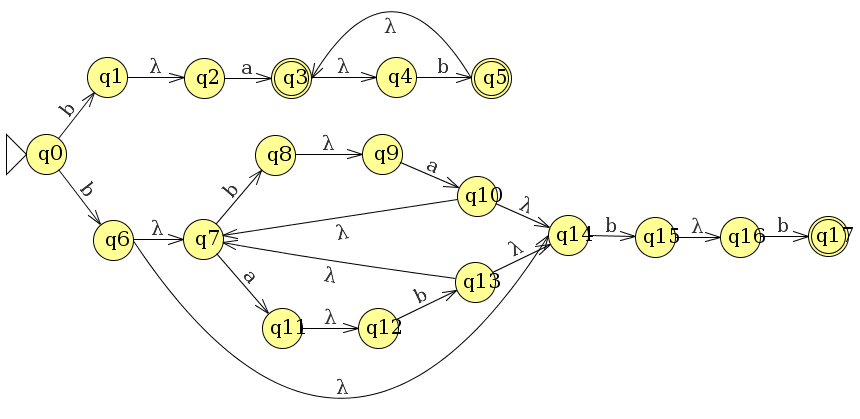
\includegraphics[width=16cm]{assets/hw_07_2a.png}
  \end{center}
  \item \( (a\cup b)(ab)^*(abb)^* \)
  \begin{center}
    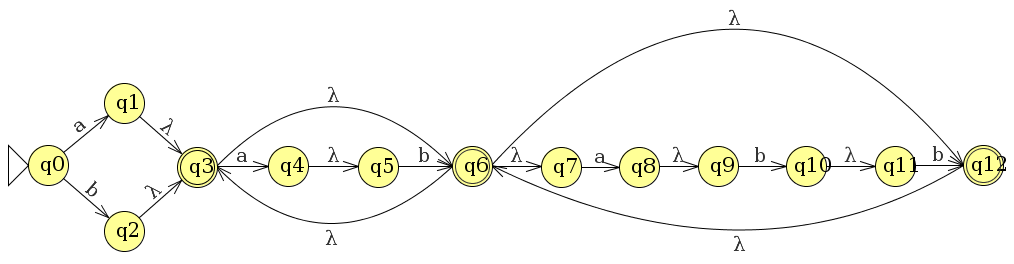
\includegraphics[width=16cm]{assets/hw_07_2b.png}
  \end{center}
\end{enumerate}

\subsection*{Problem 3}
Use the construction from Lemma 1.60 to make REs for the following DFAs. Your
resulting REs should be the exact ones that result from applying the
construction \textit{when you eliminate the states in numerical order}.
\begin{enumerate}[(a)]
  \item \( b^*aa^*\cup b^*aa^*b(ab^*aa^*b\cup ba^*b)^*ba^* \)
  \item \( a(a\cup b)\Bigg(\big((a\cup b)^2b\big)\cup\big((a\cup b)^2a(a\cup b)\big)\Bigg)^*
    (\epsilon\cup a\cup b) \)
\end{enumerate}

\begin{center}
  If you have any questions, comments, or concerns, please contact me at
  alvin@omgimanerd.tech
\end{center}

\end{document}
